\phantomsection

% Increment the chapter counter so \thechapter shows the correct number
% and make it referenceable with \ref
\refstepcounter{chapter}

% Manually add this appendix to the Table of Contents
\addcontentsline{toc}{chapter}{Apéndice \thechapter: Implementación del clúster virtualizado HTCondor}

% Add vertical space above the title (mimics standard chapter spacing)
\vspace{40pt}

% Display the actual chapter title (centered, large, bold)
{\centering \normalfont\huge\bfseries Apéndice~\thechapter: Implementación del clúster virtualizado HTCondor~\par}

% Add spacing between title and horizontal rule
\vspace{10pt}

% Draw a horizontal line across the page for visual separation
{\centering \rule{\textwidth}{0.4pt} \par}

% Add vertical space between title section and content
\vspace{40pt}

% Set the running headers for left and right pages
\markboth{Apéndice \thechapter: Implementación del clúster virtualizado HTCondor}{Apéndice \thechapter: Implementación del clúster virtualizado HTCondor}


\FloatBarrier\subsection{Instalación en un entorno virtualizado}

El clúster de computación distribuida de HTCondor actualmente soporta la versión \texttt{8.4.11}. A continuación se muestra la salida de uno de los nodos Raspberry-Pi, los cuales tienen una instalación heterogénea:

% HTCondor version output
\begin{minted}[
    frame=lines,
    framesep=2mm,
    baselinestretch=1.2,
    bgcolor=lightgray!10,
    fontsize=\footnotesize,
]{bash}
condor_version
$CondorVersion: 8.4.11 Feb 06 2017 BuildID: Debian-8.4.11~dfsg.1-1 Debian-8.4.11~dfsg.1-1
$$CondorPlatform: ARMV7L-Raspbian_ $
\end{minted}


Si bien esta versión es compatible con el \textbf{universo parallel}, la limitada documentación disponible para la version \texttt{8.4.11} en particular representó un obstáculo para implementar algoritmos que utilizaran OpenMPI. Por esta razón, y siguiendo la recomendación del asesor de este proyecto, se decidió implementar dicho universo en una infraestructura virtualizada.

\FloatBarrier\subsubsection{Infraestrutura virtualizada}

El primer paso hacia la implementación de la nueva infraestructura HTCondor fue desplegar máquinas virtuales en la infraestructura del \GRID. Para ello se utilizó un servidor dedicado que ejecuta el hipervisor \cite{xcpng_intro}, en el cual se configuraron 5 máquinas virtuales con el sistema operativo~\texttt{AlmaLinux 9.6 (Sage Margay) x86\_64}. Las máquinas pueden verse, mediante la interfaz Xen-Orchestra en la figura \ref{fig:xen-vms}. Esta configuración difiere significativamente de la arquitectura armv7l de 32 bits que utiliza el clúster de Raspberry Pi actual. La elección de este sistema operativo no fue trivial, se fundamentó en varios criterios: según la documentación oficial, AlmaLinux es uno de los sistemas operativos oficialmente soportados por HTCondor~\cite{HTCondor_install}, además de haber sido implementado exitosamente por instituciones como el CERN \citep{Bunsic2025}.

\begin{figure}
	\centering
	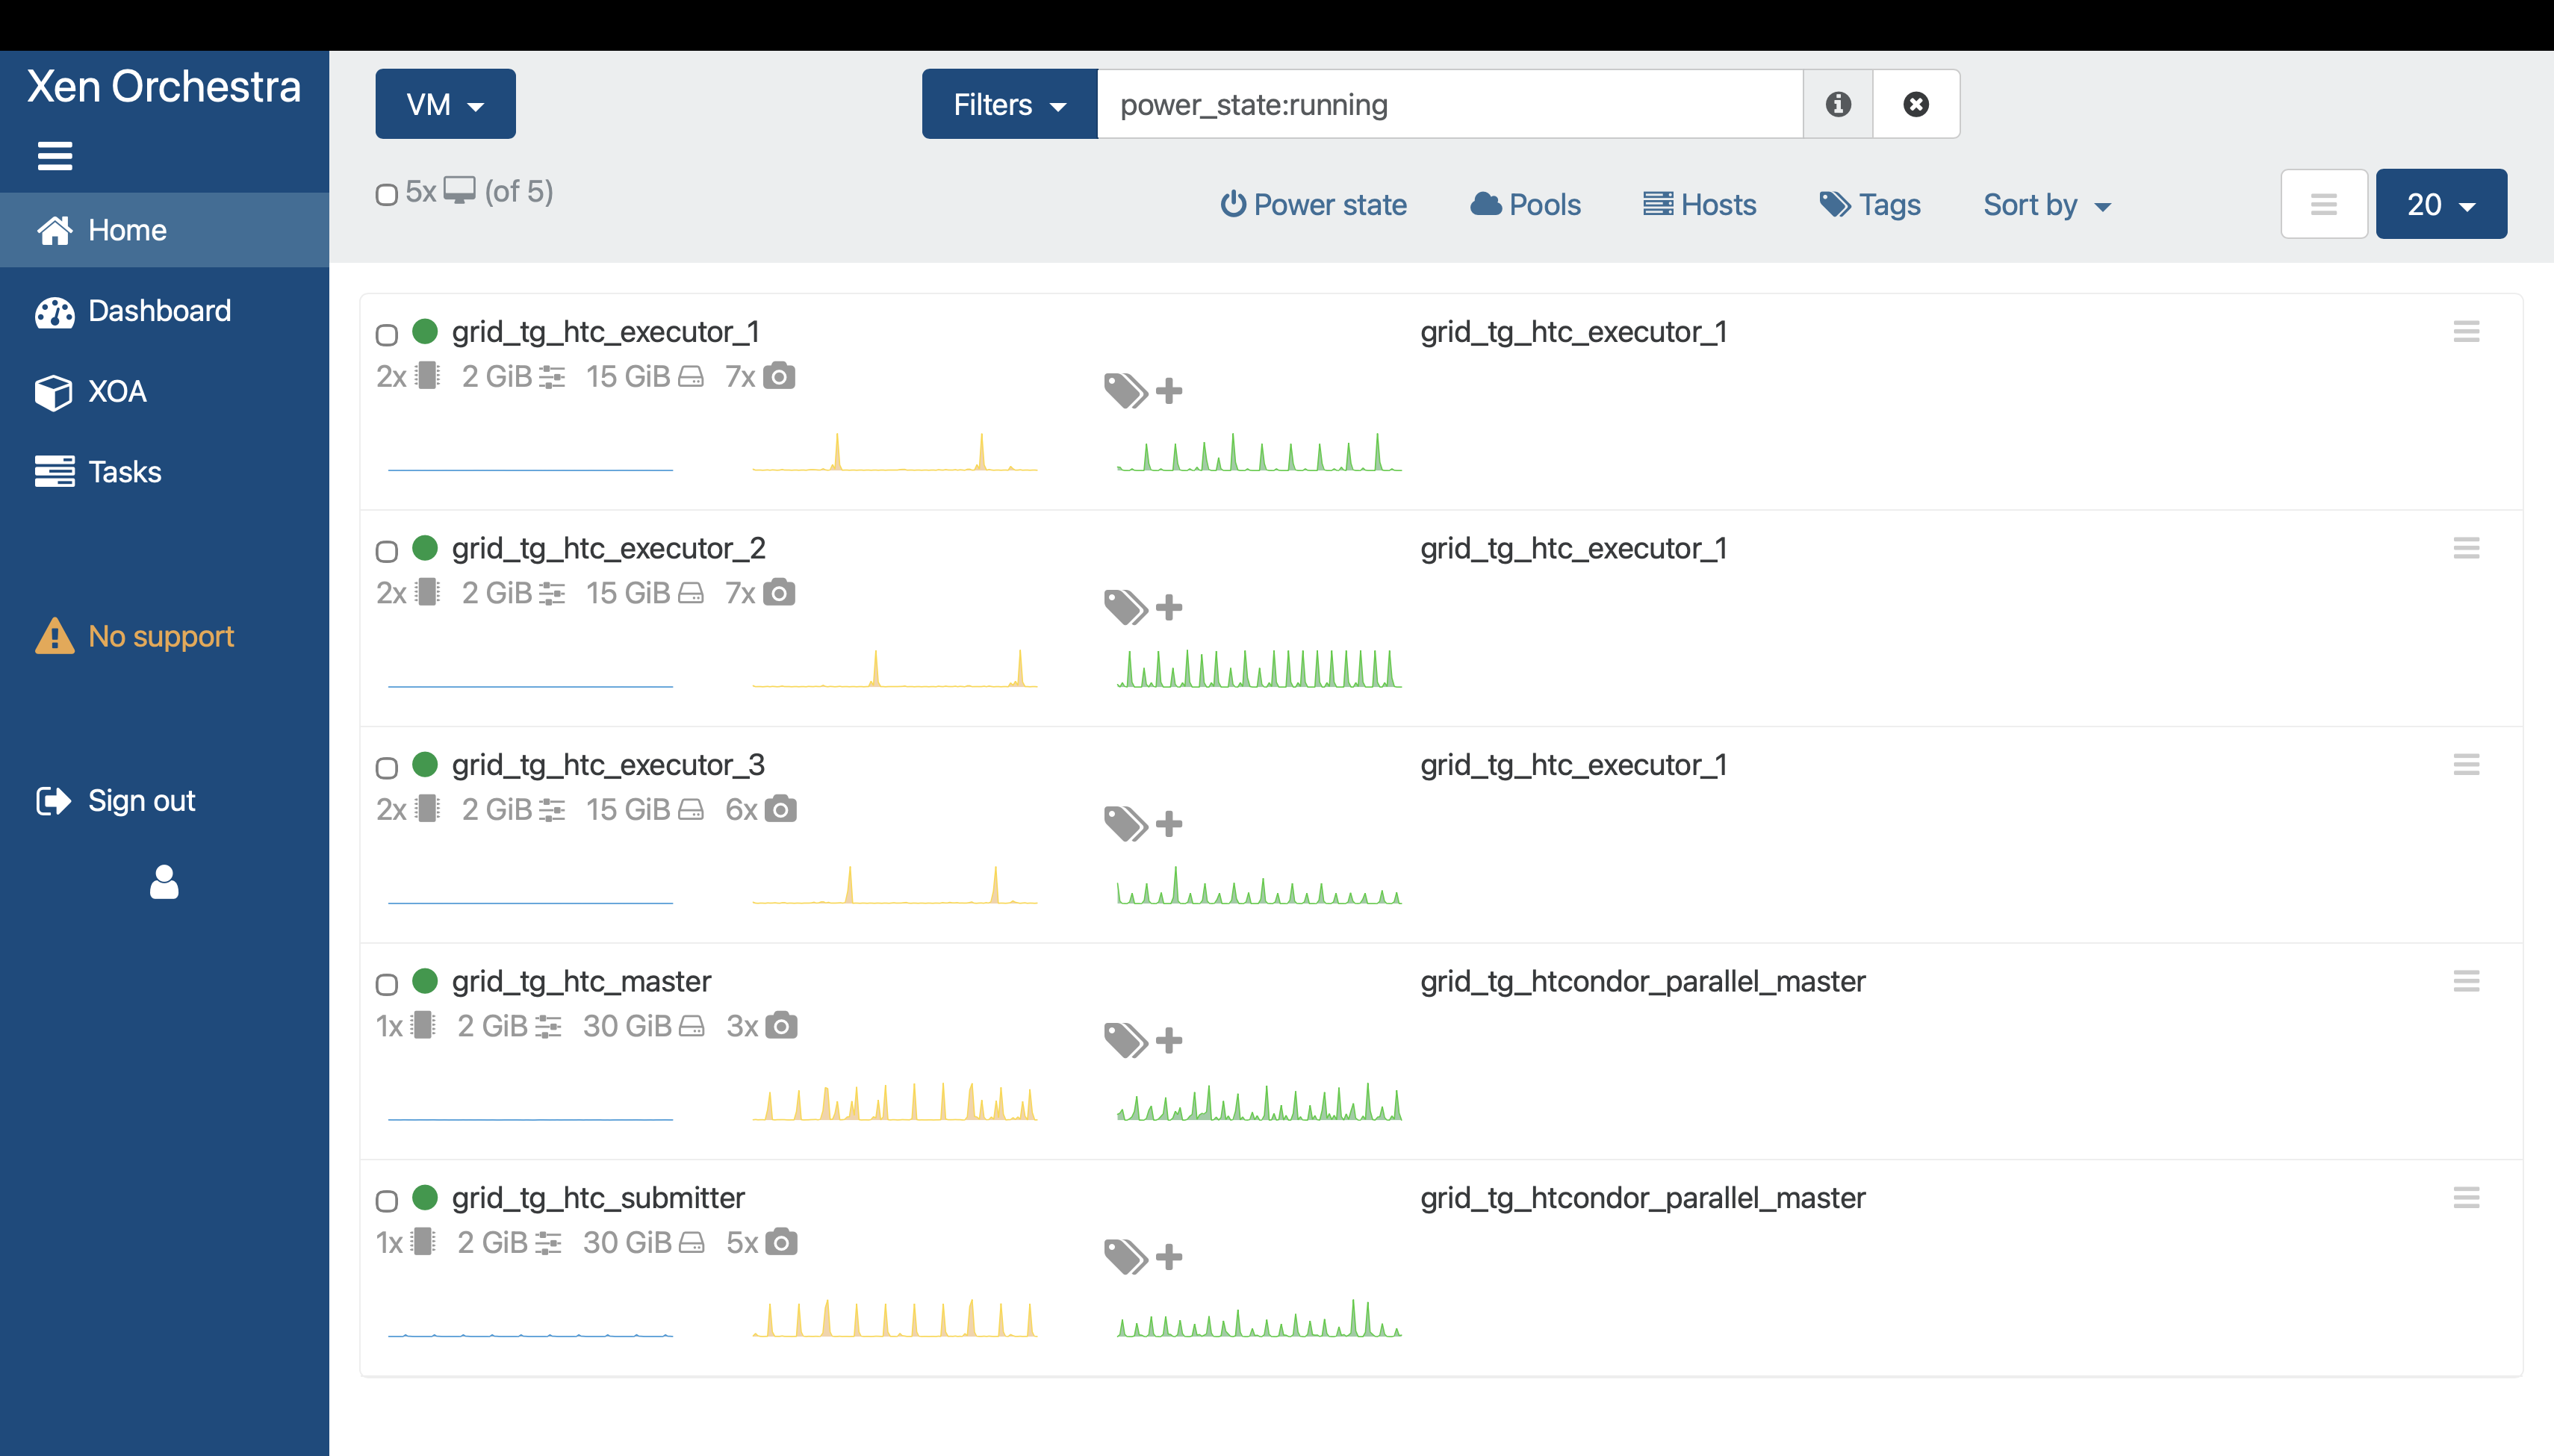
\includegraphics[scale=0.25]{apendices/infra-virtual/xen-vms.png}
	\caption{Vista de las máquinas virtuales para la nueva infraestructura HTCondor virtualizada de \GRID}
	\label{fig:xen-vms}
\end{figure}

A cada máquina se le asignó, al momento de instalación, una dirección IP dentro de la red \texttt{172.30.28.0/24} como se muestra en la Tabla~\ref{tab:nodos-htcondor}:

\begin{table}[H]
	\centering
	\renewcommand{\arraystretch}{1.2} % Espaciado reducido
	\fontsize{9pt}{10pt}\selectfont % Tamaño de fuente 9pt
	\begin{tabular}{|p{3cm}|p{3cm}|p{4.5cm}|p{2.5cm}|}  % Total: 14cm (incluyendo bordes)
		\hline
		\textbf{Rol del nodo} & \textbf{Dirección IP} & \textbf{Nombre de usuario} & \textbf{Usuario} \\ \hline
		Grid Manager          & 172.30.28.29          & gridmanager                & alma             \\ \hline
		Master                & 172.30.28.30          & master                     & alma             \\ \hline
		Submit                & 172.30.28.31          & submit                     & alma             \\ \hline
		Ejecutor 1            & 172.30.28.32          & exec01                     & alma             \\ \hline
		Ejecutor 2            & 172.30.28.33          & exec02                     & alma             \\ \hline
		Ejecutor 3            & 172.30.28.34          & exec03                     & alma             \\ \hline
	\end{tabular}
	\caption{Configuración de nodos del clúster HTCondor virtualizado}
	\label{tab:nodos-htcondor}
\end{table}


\FloatBarrier\subsubsection{Instalación de HTCondor}

Para la instalación de HTCondor se diseño el siguiente script, el cual emplea otro script que puede encontrarse en la documentación oficial \cite{HTCondor-linux-install}.



% HTCondor Install script
\begin{minted}[
    frame=lines,
    framesep=2mm,
    baselinestretch=1.2,
    bgcolor=lightgray!10,
    fontsize=\footnotesize,
]{bash}
#!/bin/bash

# Script de instalación de HTCondor para Alma Linux 9.6
# Uso: ./install-condor.sh <tipo_nodo> <hostname_master> <contraseña>
# Tipos de nodo: master, submit, worker

if [ "$#" -ne 3 ]; then
    echo "Uso: $0 <tipo_nodo> <hostname_master> <contraseña>"
    echo "Tipos de nodo: master, submit, worker"
    echo "Ejemplo: $0 master master.example.com micontraseña"
    exit 1
fi

NODE_TYPE=$1 #Tipo de nodo, hay tres opciones: {'master', 'submit' y 'worker;}
MASTER_FQN=$2 # Fully Qualified Name del nodo maestro.
PASSWORD=$3 #Deberá ser igual para todos los nodos de manera que puedan comunicarse entre sí

sudo dnf update -y

case $NODE_TYPE in
    master)
        echo "Instalando nodo MASTER..."
        curl -fsSL https://get.htcondor.org | sudo /bin/bash -s -- --no-dry-run --cm $MASTER_FQN --password $PASSWORD --channel lts
        ;;
    submit)
        echo "Instalando nodo SUBMIT (access point)..."
        curl -fsSL https://get.htcondor.org | sudo /bin/bash -s -- --no-dry-run --ap $MASTER_FQN --password $PASSWORD --channel lts
        ;;
    worker)
        echo "Instalando nodo WORKER (execution point)..."
        curl -fsSL https://get.htcondor.org | sudo /bin/bash -s -- --no-dry-run --ep $MASTER_FQN --password $PASSWORD --channel lts
        ;;
    *)
        echo "Error: Tipo de nodo inválido. Use: master, submit o worker"
        exit 1
        ;;
esac

echo "Instalación completada exitosamente!"
\end{minted}


Aparte del script anterior, tambien se creó una guía en formato.md la cual puede ser encontrada en el siguiente link:
